I have an apple, I have a pen...

Citation example, deep learning \cite{lecun2015deep} is ...

\section{Apple}

Figure \ref{fig:ch2_apple} shows an apple.

\begin{figure}[!ht]
    \centering
    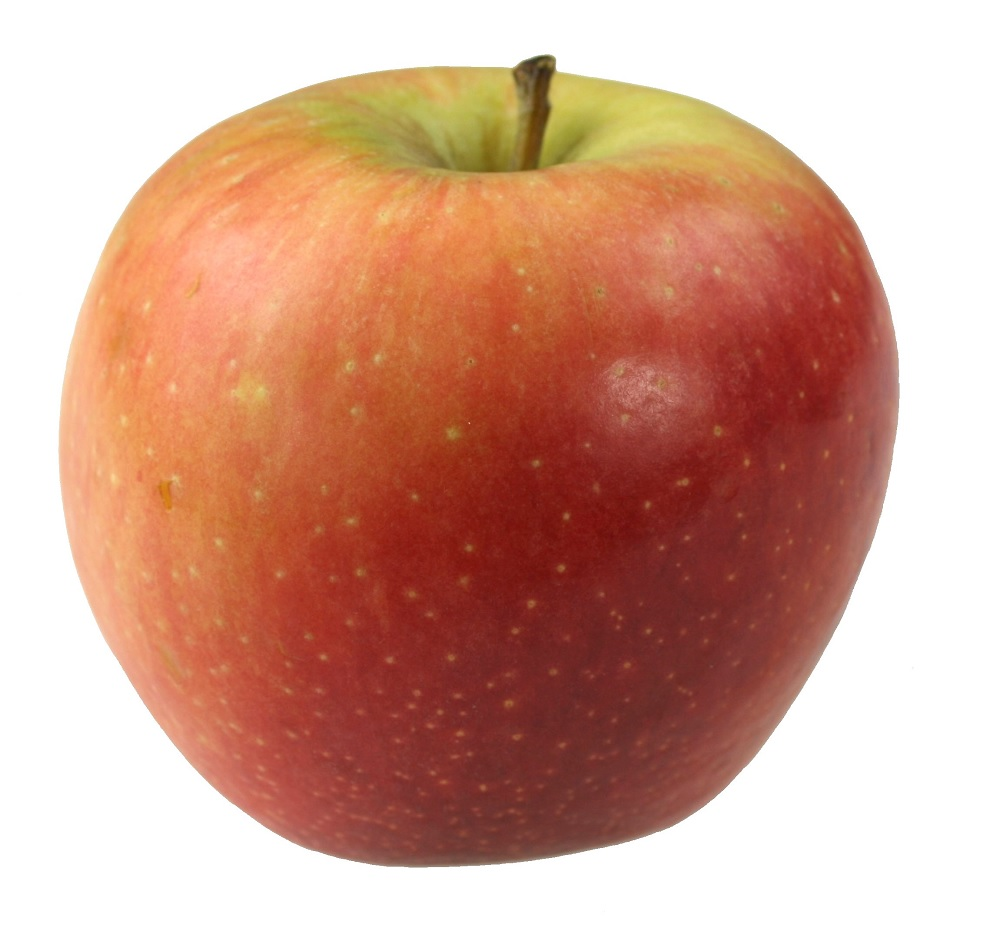
\includegraphics[width=0.3\linewidth]{Images/chapter2/apple.jpg}
    \caption[Apple]{Apple.}
    \label{fig:ch2_apple}
\end{figure}

Table \ref{tab:ch2_fruit_price} shows the apple price.

\begin{table}[ht]
\centering
\caption{Fruit Price}
\label{tab:ch2_fruit_price}
\begin{tabular}{|l|l|}
\hline
\textbf{Fruit Name} & \textbf{Price} \\ \hline
Apple               & 10             \\ \hline
\end{tabular}
\end{table}

Bigger table below

\begin{table}[ht]
\centering
\caption{Fruit Price}
\label{tab:ch2_fruit_price}
\resizebox{\columnwidth}{!}{
\begin{tabular}{|l|l|}
\hline
\textbf{Fruit Name} & \textbf{Price} \\ \hline
Apple               & 10             \\ \hline
\end{tabular}}
\end{table}